\documentclass[a4]{scrartcl}

% \usepackage[ngerman]{babel}
\usepackage[utf8]{inputenc}
\usepackage{mathtools}
\usepackage{amsmath}
\usepackage{amssymb}
\usepackage{geometry}
\usepackage{scrlayer-scrpage}
\usepackage{float}
\usepackage{xcolor}
\pagestyle{scrheadings}
\clearscrheadfoot

\usepackage[backend=biber, maxbibnames=99]{biblatex}
\addbibresource{references.bib}

\setlength{\parindent}{0cm}


\geometry{
  paper=a4paper, % Change to letterpaper for US letter
  top=2cm, % Top margin
  bottom=1.5cm, % Bottom margin
  left=2cm, % Left margin
  right=3cm, % Right margin
}

\ohead{\\
Pina Kolling\\
piko0011}

\usepackage[framemethod=TikZ]{mdframed}

% Style %
\mdfdefinestyle{enviStyle}{
   innertopmargin = 10pt,
  linewidth      = 1pt,
  frametitlerule = true,
  roundcorner    = 2pt%
}


\newenvironment{CountingDefinition}[2][]{%
   \ifstrempty{#1}%
   {\mdfsetup{%
      frametitle={{\strut ~}}}
   }%
   {\mdfsetup{%
      frametitle={{\strut ~#1}}}%
   }%
   \mdfsetup{
      nobreak                   = true,
     linecolor                 = gray,
    frametitlebackgroundcolor = gray!50,
    style                     = enviStyle
   }
   \begin{mdframed}[]\relax%
   \label{#2}}{\end{mdframed}}

\begin{document}

\section*{Summary: Lecture 6}

Summary for the chapter \textit{8.2}. \cite{CC, book}


\subsection*{Completeness}


\begin{CountingDefinition}[]{def:validLabelPlacement}
Let $C$ be a complexity class and let $L$ be a language in $C$. $L$ is called $C$\textit{-complete} if any language $L' \in C$ can be reduced to $L$.
\ \\

(Every language of a complexity class can be reduced to $L$.)
\end{CountingDefinition}



\begin{itemize}
\item reducitbility is transitive $\rightarrow$ problems are ordered by difficulty
\item complete problems can capture the difficulty of a class
\item problem is seen as cpmpletely understood if the problem is complete
\end{itemize}


\color{violet} \textbf{Question: }

Which problems can be reduced to a formal language? 
\begin{itemize}
\item[] \color{black}
\textsc{Sat} can be expressed as formal language. \cite{lang} \\
$\Rightarrow$ \textsc{Sat} can be reduced to a formal language. (?) \\
\textsc{Sat} is in NP. \cite{book}
\ \\

Because \textsc{Circuit Sat} can be reduced to \textsc{Sat}: \textsc{Circuit Sat} can be reduced to a formal language. (?)
\textsc{Circuit Sat} is NP-complete. \cite{wiki} \\
Any formal language $L \in$ NP can be reduced to \textsc{Circuit Sat}? OR the other way around?
\ \\

\begin{CountingDefinition}[Formal language]{def:validLabelPlacement}
Formal languages are abstract languages, which define the syntax of the words that get accepted by that language. It is a set of words that get accepted by the language and has a set of symbols that is called alphabet, which contains all the possible characters of the words. Those characters are called nonterminal symbols. \cite{CNF, language}
\ \\

\textbf{Kleene star} \\
The Kleene star $\Sigma^*$ of an alphabet $\Sigma$ is the set of all words that can be created through concatenation of the symbols of the alphabet $\Sigma$. The empty word $\epsilon$ is included. 
\ \\

\textbf{Formal language}\\
A formal language $L$ over an alphabet $\Sigma$ is a subset of the Kleene star of the alphabet: $L \subseteq \Sigma^*$
\end{CountingDefinition}

Where to set the line between lanuguage decisions and other problems? Can every problem be contrcuted as a formal language?
\ \\

Is everything that is reducable to \textsc{Sat} reducable to a formal language because of the transitivity?
\ \\

I assume it does not have an influence on the complexity of a problem if it can be expressed as a formal language? Are formal languages part of specific complexity classes?

\end{itemize}

\color{black}



\begin{CountingDefinition}[Closed under reduction]{def:validLabelPlacement}
The following complexity classes are all closed under reductions:
\begin{itemize}
\item[] \textsc{P} \ \ \  \textsc{NP} \ \ \ \textsc{coNP}
\ \ \ \textsc{L}
\ \ \  \textsc{NL}
\ \ \  \textsc{PSPACE}
\ \ \ \textsc{EXP}
\end{itemize}

A class $C$ is closed under reductions if whenever $L$ is reducible to $L'$ and $L' \in C'$, then $L \ in C'$.
\ \\

If a complete problem in $C$ belongs in a class $C' \subseteq C$, $C = C'$.

\end{CountingDefinition}


\begin{figure}[H]
\begin{center}
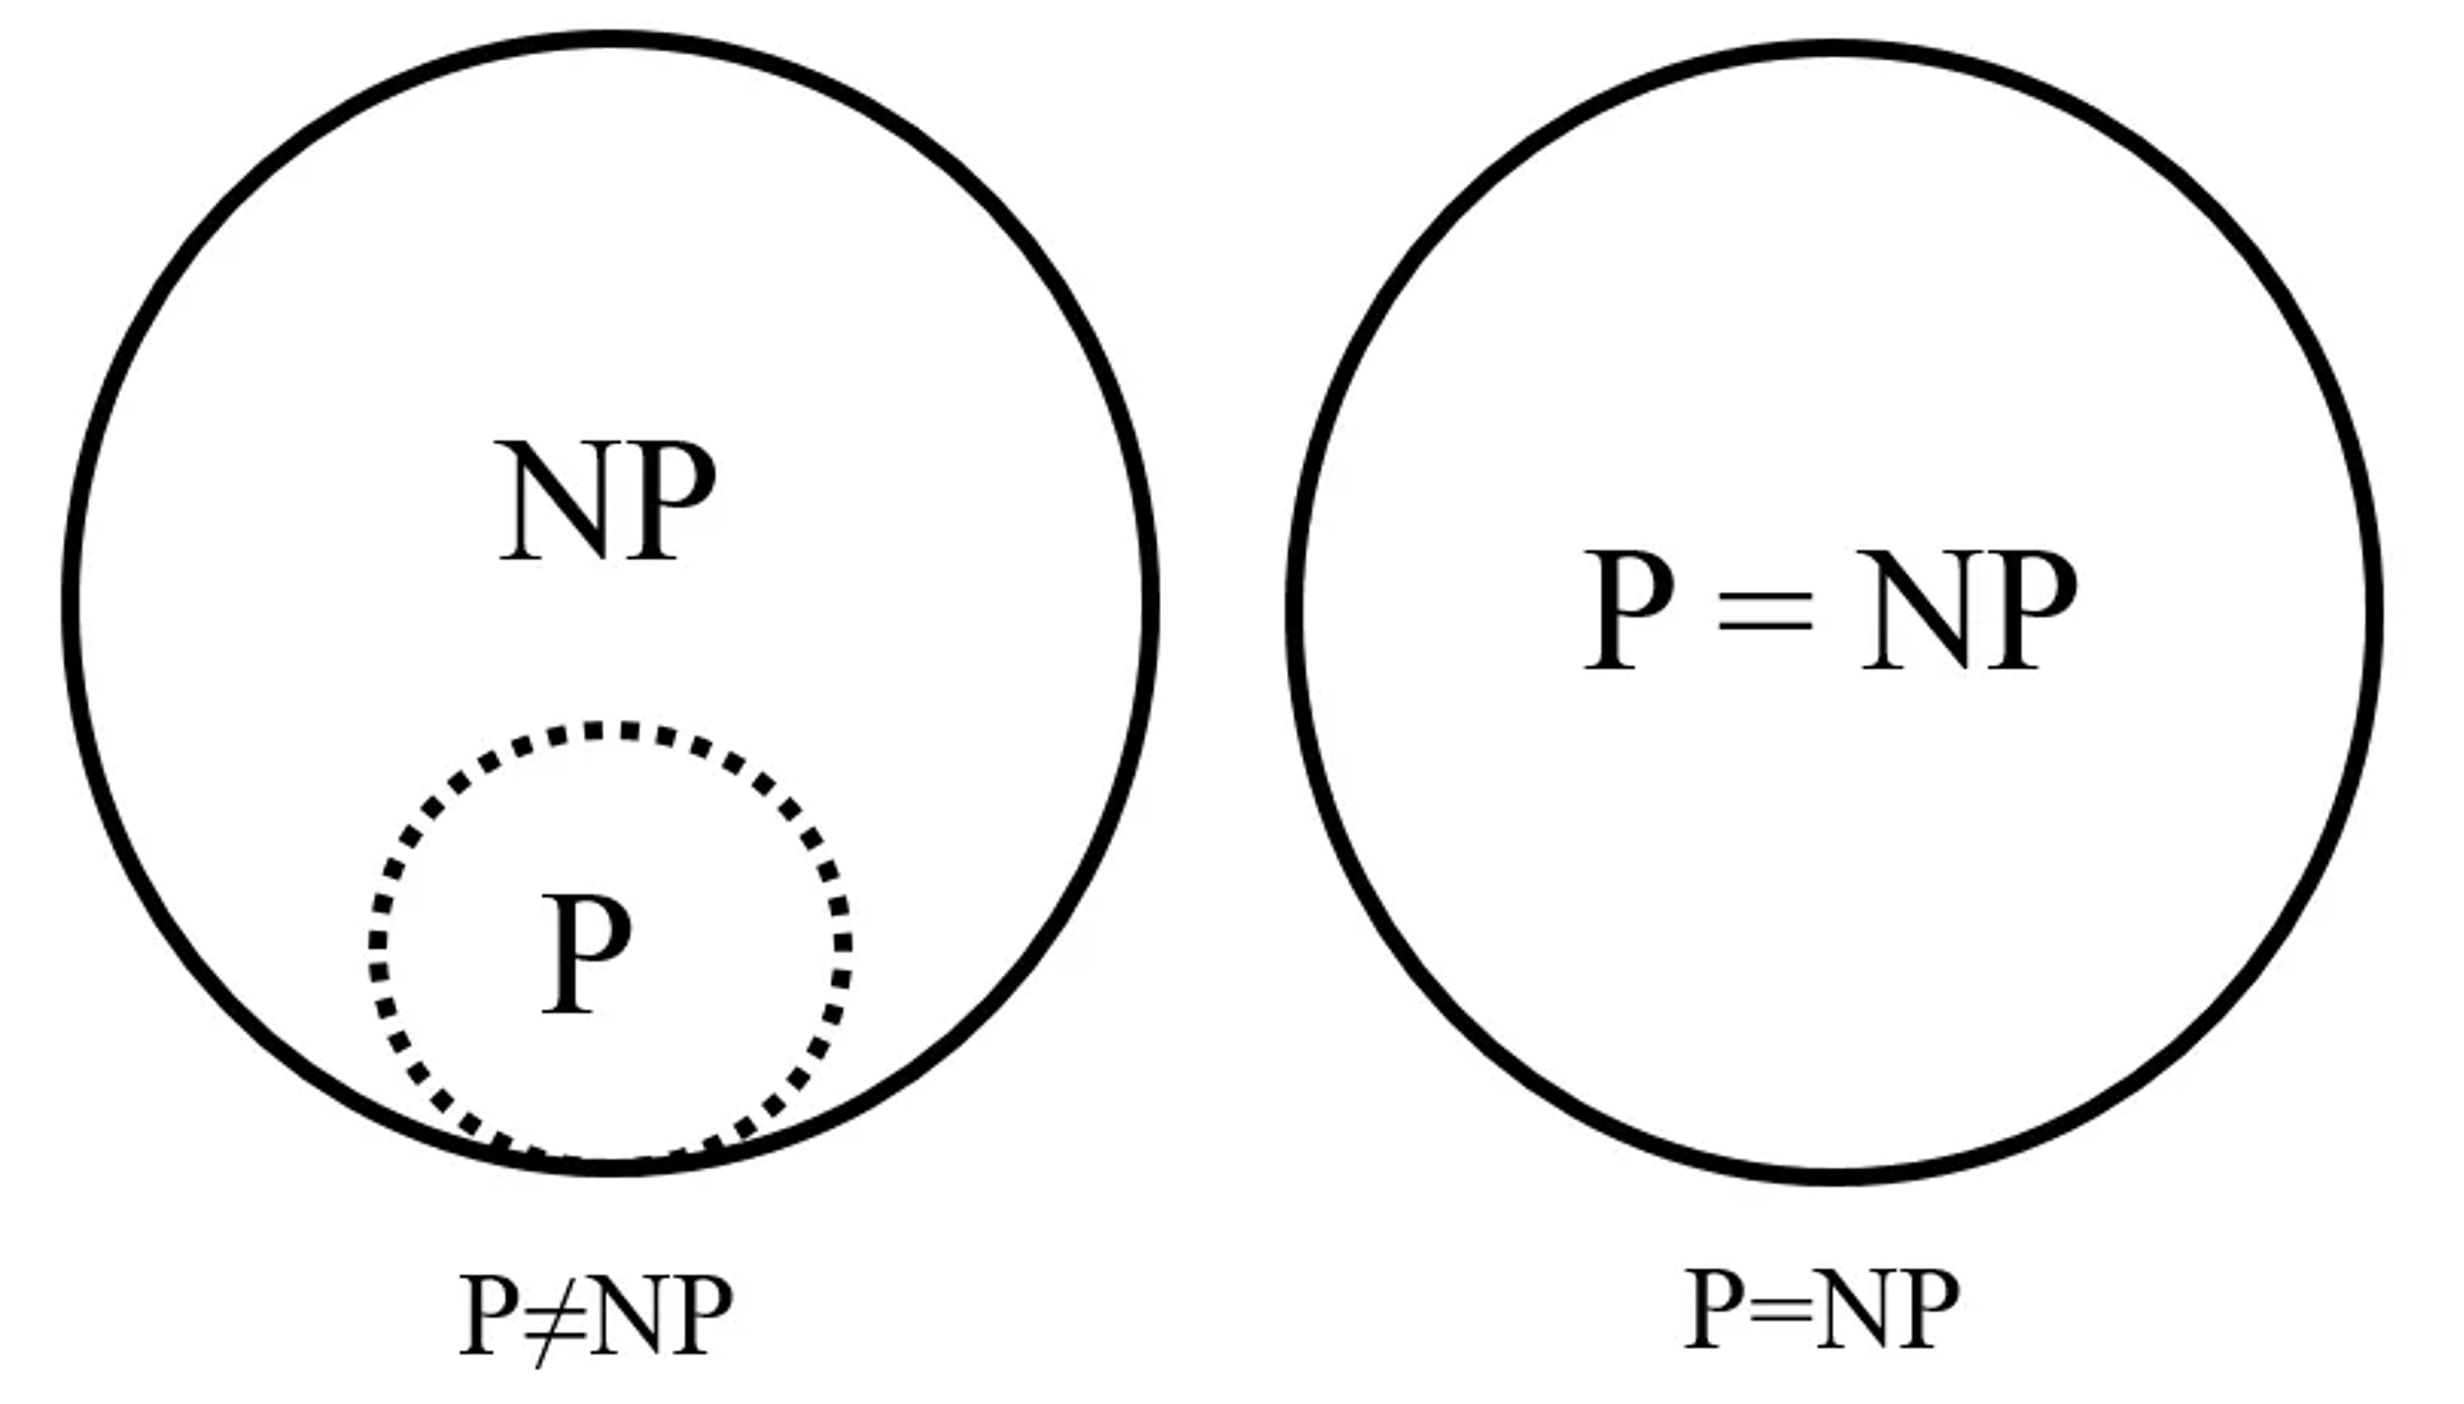
\includegraphics[scale=0.2]{PNP.jpg}
\hspace*{5em}
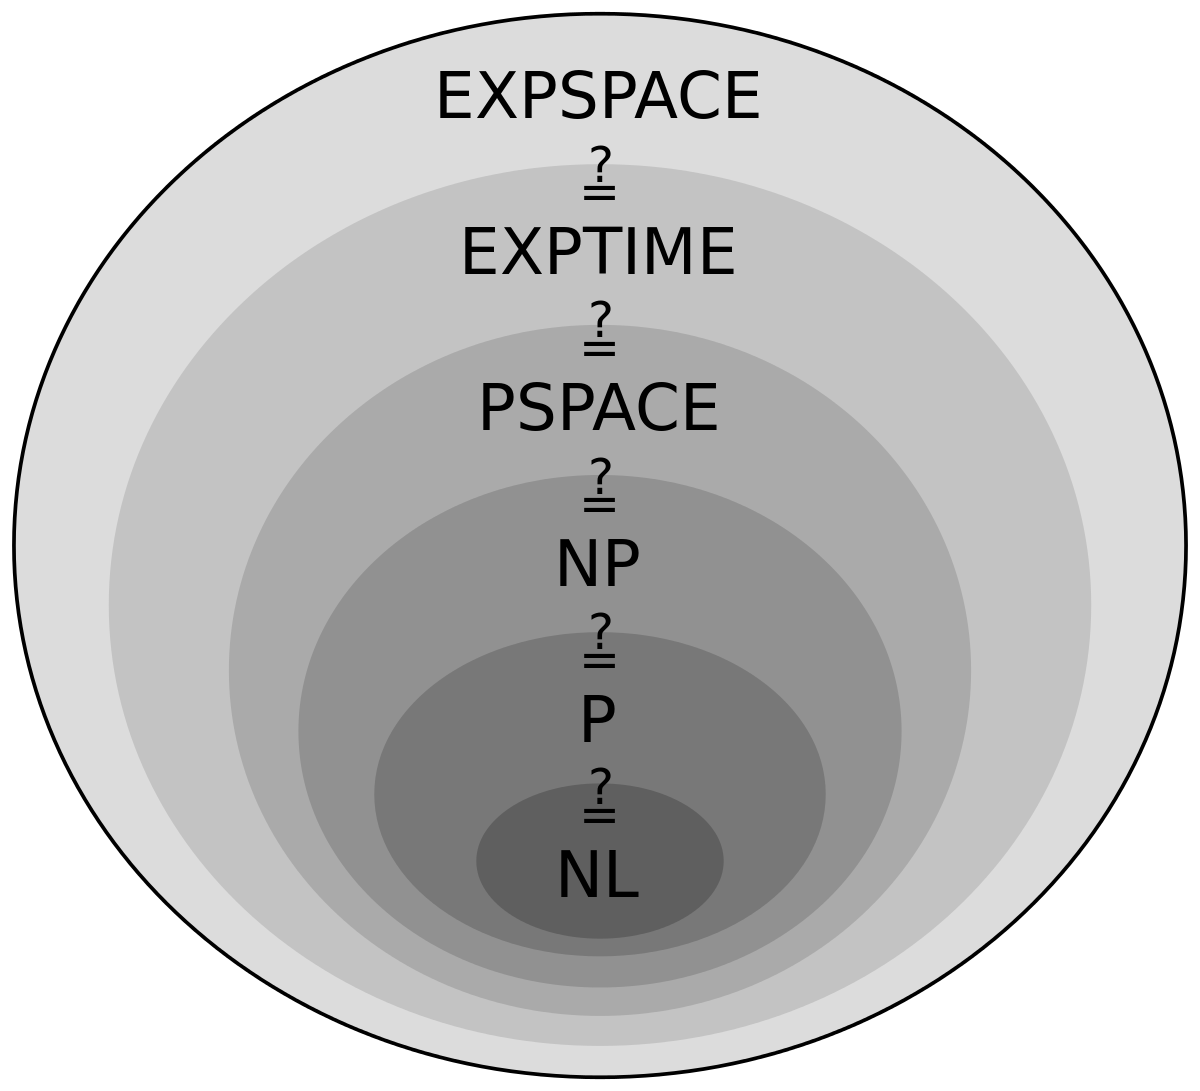
\includegraphics[scale=0.15]{classes.png}
\end{center}
\caption{P and NP sets \cite{PNPsets} and complexity classes \cite{classesPic}}
\end{figure}




\begin{itemize}

\item examples: 
\begin{itemize}
\item if an NP-complete language is in P, then NP = P 
\item if a P-complete language is in L, then P = L
\item if a P-complete language is in NL, then P = NL
\item no EXP-complete language can be in P
\end{itemize}

\end{itemize}

%\subsection*{Table method -- time complexity}

%\begin{itemize}
%\item table method to understand time complexity
%\end{itemize}




\subsection*{\textsc{P}-completeness of \textsc{CircuitValue}}

\begin{CountingDefinition}[Problem: \textsc{CircuitValue}]{def:validLabelPlacement}
The \textsc{CircuitValue} Problem is the problem of computing the output of a given Boolean circuit on a given input.
\ \\

In terms of time complexity, it can be solved in linear time (topological sort).
\end{CountingDefinition}

\begin{itemize}
\item \textsc{P}-complete
\end{itemize}

\textbf{Proof idea:}

\begin{itemize}
\item \textsc{CircuitValue} is in P (prerequisite for being P-complete)
\item show: any language $L \in $ P can be reduced to \textsc{CircuitValue}

\end{itemize}



\color{red} TODO \\
proof! \\
\color{black}
\color{violet} Questions:
\color{black}






\subsection*{\textsc{CicuitSat} is \textsc{NP}-complete}

\begin{CountingDefinition}[Problem: \textsc{CircuitSat}]{def:validLabelPlacement}
The circuit satisfiability problem (\textsc{CircuitSat}) is the decision problem of determining whether a given Boolean circuit has an assignment of its inputs that makes the output true.
\ \\

Input: a Boolean circuit $C$ 
\ \\

Question: Is there a truth assignment which makes $C$ output the value true?
\end{CountingDefinition}

\begin{itemize}
\item cook's theorem: \textsc{CircuitSat} is \textsc{NP}-complete
\end{itemize} 
\textbf{Proof idea:}
\begin{itemize}
\item circuit decides nondeterministically (?)
\item a variable is added in the nondeterministic Turing Machine
\item check if one of the variables is tue: use this choice (?)
\item problem: can we set thiese variables such that the Turing Machine accepts?
\item answer corresponds direct to \textit{is there a choice of nd decisions such that the turing machine accepts?}
\item extremely direct reduction
\item \textsc{SAT} is \textsc{NP}-complete
\end{itemize}




\color{red} TODO \\
proof! \\
\color{violet} Questions:
\color{black}



\begin{CountingDefinition}[Relation between complexity classes]{def:validLabelPlacement}
$N \subseteq NL \subseteq NC \subseteq P \subseteq NP \subseteq PSPACE$
\end{CountingDefinition}

\color{red} TODO \\
\color{black}


\subsection*{NP-complete problems}

\begin{figure}[H]
\begin{center}
\includegraphics[scale=0.6]{NP_complete.png}
\end{center}
\caption{NP-complete problems in relation}
\end{figure}


\begin{itemize}
\item $k$-\textsc{SAT} for $k \geq 3$ is NP-complete
\end{itemize}

\begin{CountingDefinition}[\textsc{Circuit-SAT}]{def:validLabelPlacement}
The circuit satisfiability problem (\textsc{Circuit-SAT}) is the decision problem of determining whether a given Boolean circuit has an assignment of its inputs that makes the output true.
\end{CountingDefinition}


\begin{CountingDefinition}[\textsc{SAT}]{def:validLabelPlacement}
The \textsc{SAT} (satisfiability) problem is the problem of determining if there exists an interpretation that satisfies a given Boolean formula. \cite{GTI}
\end{CountingDefinition}


\begin{CountingDefinition}[\textsc{3-SAT}]{def:validLabelPlacement}
Like the \textsc{SAT} problem, \textsc{3-SAT} is determining the satisfiability of a formula in CNF where each clause is limited to at most three literals.
\end{CountingDefinition}


\begin{CountingDefinition}[\textsc{Clique}]{def:validLabelPlacement}
The \textsc{Clique} problem is the problem of finding cliques (subsets of vertices, all adjacent to each other, also called complete subgraphs) in a graph.
\end{CountingDefinition}


\begin{CountingDefinition}[\textsc{VertexCover}]{def:validLabelPlacement}
In graph theory, a \textsc{VertexCover} (sometimes \textsc{NodeCover}) of a graph is a set of vertices that includes at least one endpoint of every edge of the grap
\end{CountingDefinition}


\begin{CountingDefinition}[\textsc{HamiltonCycle}]{def:validLabelPlacement}
A \textsc{HamiltonCycle} is a graph cycle (i.e., closed loop) through a graph that visits each node exactly once.
\end{CountingDefinition}


\begin{CountingDefinition}[\textsc{TravellingSalesman}]{def:validLabelPlacement}
\textit{Given a list of cities and the distances between each pair of cities, what is the shortest possible route that visits each city exactly once and returns to the origin city?}
\end{CountingDefinition}


\begin{CountingDefinition}[\textsc{GraphColoring}]{def:validLabelPlacement}
In graph theory, graph coloring is a special case of graph labeling. It is an assignment of colors to elements of a graph subject to certain constraints.
\end{CountingDefinition}


\begin{CountingDefinition}[\textsc{ExactCover}]{def:validLabelPlacement}
Given a collection $S$ of subsets of set $X$, an exact cover is the subset $S^*$ of $S$ such that each element of $X$ is contained is exactly one subset of $S^*$.
\end{CountingDefinition}


\begin{CountingDefinition}[\textsc{Knapsack}]{def:validLabelPlacement}
\textit{Given a set of items, each with a weight and a value, determine the number of each item to include in a collection so that the total weight is less than or equal to a given limit and the total value is as large as possible.}
\end{CountingDefinition}


\begin{CountingDefinition}[\textsc{SubsetSum}]{def:validLabelPlacement}
The \textsc{SubsetSum} problem involves determining whether or not a subset from a list of integers can sum to a target value. For example, consider the list of $nums = [1, 2, 3, 4]$ . If the target is 7 , there are two subsets that achieve this sum: $\{ 3, 4 \}$ and $\{ 1, 2, 4\}$.
\end{CountingDefinition}





\subsection*{P-complete problems}

\begin{itemize}
\item \textsc{CircuitValue}
\item \textsc{LinearProgramming}
\item \textsc{HornSAT}
\end{itemize}

\begin{CountingDefinition}[\textsc{CircuitValue}]{def:validLabelPlacement}
The \textsc{CircuitValue} Problem is the problem of computing the output of a given Boolean circuit on a given input.

In terms of time complexity, it can be solved in linear time (topological sort).


The problem is closely related to the \textsc{Sat} (Boolean Satisfiability) problem which is complete for NP and its complement, which is complete for co-NP.
\end{CountingDefinition}


\begin{CountingDefinition}[\textsc{LinearProgramming}]{def:validLabelPlacement}

\end{CountingDefinition}


\begin{CountingDefinition}[\textsc{HornSAT}]{def:validLabelPlacement}

\end{CountingDefinition}

\color{red} TODO \\
\color{black}



\subsection*{NL problems}

\begin{itemize}
\item \textsc{2-Sat}
\item \textsc{Reachability}
\end{itemize}


\begin{CountingDefinition}[\textsc{2-Sat}]{def:validLabelPlacement}

\end{CountingDefinition}


\begin{CountingDefinition}[\textsc{Reachability}]{def:validLabelPlacement}
Given a graph $G$ and two nodes $n_1, n_2 \in V$, is there  path from $n_1$ to $n_2$?

A graph $G=(V, E)$ is a finite set $V$ of nodes and a set $E$ of edges as node pairs.
\ \\

\textsc{Reachability} can be nondeterministically solved in space $\log n$.
\end{CountingDefinition}

\color{red} TODO \\
\color{black}



\subsection*{L problems}

\begin{itemize}
\item \textsc{1-Sat}
\end{itemize}


\begin{CountingDefinition}[\textsc{1-Sat}]{def:validLabelPlacement}

\end{CountingDefinition}


\color{red} TODO \\
\color{black}




\newpage

\printbibliography




\end{document}